\chapter{Fundamentação Teórica e Trabalhos Relacionados}

Neste capítulo são discutidos os conceitos básicos ao entendimento deste trabalho, abrangendo aprendizagem de máquina, processamento digital de imagens, segmentação de imagens e extração de características.

\section{Aprendizagem de máquina e reconhecimento de padrões}

Conforme \cite{alpaydin:2010}, aprendizagem de máquina é uma área da inteligência artificial que estuda métodos computacionais, a fim de obter um determinado conhecimento específico através de experiências. A aplicação prática de aprendizado de máquina inclui o processamento de linguagem natural, diagnósticos médicos, detecção de intrusos, entre outros. Um sistema de aprendizado tem a função de analisar informações e generalizá-las, para a extração de novos conhecimentos.

Segundo \cite{russell:2010}, os tipos de aprendizagem podem ser classificados de acordo com o tipo de \textit{feedback} que recebem do ambiente:

\begin{itemize}
    \item \textbf{Aprendizagem não-supervisionada}: o agente aprende padrões na entrada, embora não seja fornecido nenhum \textit{feedback} explícito. A tarefa mais comum de aprendizagem não-supervisionada é o agrupamento, ou seja, a detecção de grupos de exemplos de entrada potencialmente úteis.
    \item \textbf{Aprendizagem por reforço}: também conhecida como aprendizagem semi-supervisionada. O agente aprende a partir de uma série de reforços - recompensas ou punições.
    \item \textbf{Aprendizagem supervisionada}: o agente observa alguns exemplos de pares de entrada e saída, e aprende uma função que faz o mapeamento da entrada para a saída. 
\end{itemize}

Os problemas de aprendizagem podem ainda ser divididos de acordo com o tipo de saída que demandam:

\begin{itemize}
	\item \textbf{Problemas de classificação}: quando a saída esperada para o problema é uma classe ou categoria, ou seja, um valor discreto;
	\item \textbf{Problemas de regressão}: quando a saída esperada para o é um valor numérico, normalmente contínuo.
\end{itemize}

Um problema de classificação, ou seja, um problema em que o objetivo é atribuir corretamente classes discretas (rótulos) aos exemplos de dados, consiste na determinação de regras e posterior classificação desses exemplos. Este conjunto de regras é criado por um classificador, que recebe como entrada um vetor de características e oferece como saída uma classe resultante para a instância que as características descrevem, conforme pode ser visto na figura \ref{fig:classificador}.

\begin{figure}[h!]
  \centering
  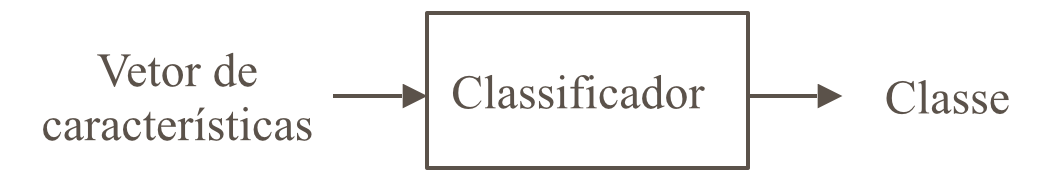
\includegraphics[width=0.7\textwidth]{imgs/classificador}
  \caption{Representação de classificador como uma função de bloco}
  \label{fig:classificador}
\end{figure}

Os tipos de classificadores utilizados neste trabalho serão discutidos com mais detalhes na seção \ref{sec:classificacao}.

Para composição do modelo de aprendizagem, uma base de dados de treinamento é utilizada. Esta base deve possuir uma quantidade significativa e com boa representatividade das classes envolvidas no problema. Normalmente se usa uma parte da base de dados de treinamento para validação do modelo de aprendizado (validação cruzada) ou mesmo uma base de dados diferente (base de testes ou validação), para que indicadores de qualidade do modelo possam ser avaliados. A seção \ref{sec:avaliacao} discorre sobre os métodos de avaliação utilizados neste trabalho.

Técnicas de aprendizagem de máquina podem ser utilizadas para encontrar padrões em diversos domínios, inclusive em imagens. É neste ponto que a disciplina de aprendizagem de máquina, advinda da área de inteligência artificial, se encontra com a disciplina de reconhecimento de padrões, advinda da área de processamento de sinais. Segundo \cite{jain:1989}, o fluxo padrão para soluções de reconhecimento de padrões consiste em três etapas:

\begin{enumerate}
    \item Filtragem e pré-processamento da entrada;
    \item Extração e seleção de características;
    \item Classificação.
\end{enumerate}

%%%%%%%%%%%%%%%%%%%%%%%%%%%%%%%%%%%%%%%%%%%%%%%%%

\subsection{Filtragem e Pré-processamento}

A etapa de filtragem e pré-processamento é responsável pela escolha e montagem da base de dados que será usada no processo de aprendizagem.

%TODO Reaproveitar: Em aprendizado relacionado a imagens, essa etapa é comumente a responsável por normalizar e salientar as características desejadas nas amostras (realce de imagens, filtragem, etc). Nesta etapa, dados irrelevantes, redundantes ou distorcidos são eliminados.

\subsection{Extração de Características}

A extração de características é feita selecionando os atributos oriundos dos dados (imagens, no trabalho em questão), a fim de encontrar as características úteis para o processo de reconhecimento. Essa etapa é crítica ao sucesso do aprendizado, uma vez que bons algoritmos de aprendizado só obtém êxito com uma bom conjunto de características relevantes ao problema.

\subsection{Classificação}\label{sec:classificacao}

Nesta etapa, todas as amostras de treinamento são classificadas e um modelo de aprendizado é gerado. Posteriormente ao processo de aprendizado, é nesta mesma etapa que as amostras não classificadas (ou rotuladas) receberão uma classe dentre as envolvidas no problema. É neste momento que podemos comparar o desempenho de diferentes algoritmos de aprendizado para o conjunto de características escolhidos para representar o problema. Comumente, o percentual de acerto obtido na classificação das amostras não rotuladas é um importante parâmetro para medir a acurácia do método.

São muitos os exemplos de classificadores que existem na literatura. Alguns dos mais utilizados são: classificadores estatísticos, redes neurais artificiais, árvores de decisão, máquinas de vetores de suporte, KNN, etc \cite{jain:1989}.

Os algoritmos utilizados neste trabalho serão discutidos no capítulo \ref{cap:metodologia}

%Os algoritmos utilizados em problemas de classificação podem ser categorizados em:

%\begin{itemize}
%	\item \textbf{Probabilísticos}:
%	\item \textbf{Geométicos}:
%	\item \textbf{Simbólicos}:
%\end{itemize}

% TODO O que são conjuntos de classificadores?
% TODO falar dos essembles e etc.

%Existe uma grande variedade de algoritmos de aprendizagem de máquina propostos na literatura tais como Árvores de Decisão, k Vizinhos mais Próximos (kNN), Redes Neurais Artificiais, Support Vector Machines (SVM), etc. [Santos, 2008]. Além desses métodos individuais, os algoritmos de aprendizagem de máquina podem também ser combinados em conjuntos de classificadores [Dietterich, 2000].


\subsection{Avaliação}\label{sec:avaliacao}

Dentre indicadores importantes para a avaliação do modelo de aprendizagem criado estão: a acurácia, ou seja, o percentual de exemplos na base de validação que são classificados corretamente pelo modelo criado; a variância, que é o quanto a acurácia varia entre diferentes bases de validação;

